% Options for packages loaded elsewhere
\PassOptionsToPackage{unicode}{hyperref}
\PassOptionsToPackage{hyphens}{url}
%
\documentclass[
]{article}
\usepackage{amsmath,amssymb}
\usepackage{iftex}
\ifPDFTeX
  \usepackage[T1]{fontenc}
  \usepackage[utf8]{inputenc}
  \usepackage{textcomp} % provide euro and other symbols
\else % if luatex or xetex
  \usepackage{unicode-math} % this also loads fontspec
  \defaultfontfeatures{Scale=MatchLowercase}
  \defaultfontfeatures[\rmfamily]{Ligatures=TeX,Scale=1}
\fi
\usepackage{lmodern}
\ifPDFTeX\else
  % xetex/luatex font selection
\fi
% Use upquote if available, for straight quotes in verbatim environments
\IfFileExists{upquote.sty}{\usepackage{upquote}}{}
\IfFileExists{microtype.sty}{% use microtype if available
  \usepackage[]{microtype}
  \UseMicrotypeSet[protrusion]{basicmath} % disable protrusion for tt fonts
}{}
\makeatletter
\@ifundefined{KOMAClassName}{% if non-KOMA class
  \IfFileExists{parskip.sty}{%
    \usepackage{parskip}
  }{% else
    \setlength{\parindent}{0pt}
    \setlength{\parskip}{6pt plus 2pt minus 1pt}}
}{% if KOMA class
  \KOMAoptions{parskip=half}}
\makeatother
\usepackage{xcolor}
\usepackage[margin=1in]{geometry}
\usepackage{color}
\usepackage{fancyvrb}
\newcommand{\VerbBar}{|}
\newcommand{\VERB}{\Verb[commandchars=\\\{\}]}
\DefineVerbatimEnvironment{Highlighting}{Verbatim}{commandchars=\\\{\}}
% Add ',fontsize=\small' for more characters per line
\usepackage{framed}
\definecolor{shadecolor}{RGB}{248,248,248}
\newenvironment{Shaded}{\begin{snugshade}}{\end{snugshade}}
\newcommand{\AlertTok}[1]{\textcolor[rgb]{0.94,0.16,0.16}{#1}}
\newcommand{\AnnotationTok}[1]{\textcolor[rgb]{0.56,0.35,0.01}{\textbf{\textit{#1}}}}
\newcommand{\AttributeTok}[1]{\textcolor[rgb]{0.13,0.29,0.53}{#1}}
\newcommand{\BaseNTok}[1]{\textcolor[rgb]{0.00,0.00,0.81}{#1}}
\newcommand{\BuiltInTok}[1]{#1}
\newcommand{\CharTok}[1]{\textcolor[rgb]{0.31,0.60,0.02}{#1}}
\newcommand{\CommentTok}[1]{\textcolor[rgb]{0.56,0.35,0.01}{\textit{#1}}}
\newcommand{\CommentVarTok}[1]{\textcolor[rgb]{0.56,0.35,0.01}{\textbf{\textit{#1}}}}
\newcommand{\ConstantTok}[1]{\textcolor[rgb]{0.56,0.35,0.01}{#1}}
\newcommand{\ControlFlowTok}[1]{\textcolor[rgb]{0.13,0.29,0.53}{\textbf{#1}}}
\newcommand{\DataTypeTok}[1]{\textcolor[rgb]{0.13,0.29,0.53}{#1}}
\newcommand{\DecValTok}[1]{\textcolor[rgb]{0.00,0.00,0.81}{#1}}
\newcommand{\DocumentationTok}[1]{\textcolor[rgb]{0.56,0.35,0.01}{\textbf{\textit{#1}}}}
\newcommand{\ErrorTok}[1]{\textcolor[rgb]{0.64,0.00,0.00}{\textbf{#1}}}
\newcommand{\ExtensionTok}[1]{#1}
\newcommand{\FloatTok}[1]{\textcolor[rgb]{0.00,0.00,0.81}{#1}}
\newcommand{\FunctionTok}[1]{\textcolor[rgb]{0.13,0.29,0.53}{\textbf{#1}}}
\newcommand{\ImportTok}[1]{#1}
\newcommand{\InformationTok}[1]{\textcolor[rgb]{0.56,0.35,0.01}{\textbf{\textit{#1}}}}
\newcommand{\KeywordTok}[1]{\textcolor[rgb]{0.13,0.29,0.53}{\textbf{#1}}}
\newcommand{\NormalTok}[1]{#1}
\newcommand{\OperatorTok}[1]{\textcolor[rgb]{0.81,0.36,0.00}{\textbf{#1}}}
\newcommand{\OtherTok}[1]{\textcolor[rgb]{0.56,0.35,0.01}{#1}}
\newcommand{\PreprocessorTok}[1]{\textcolor[rgb]{0.56,0.35,0.01}{\textit{#1}}}
\newcommand{\RegionMarkerTok}[1]{#1}
\newcommand{\SpecialCharTok}[1]{\textcolor[rgb]{0.81,0.36,0.00}{\textbf{#1}}}
\newcommand{\SpecialStringTok}[1]{\textcolor[rgb]{0.31,0.60,0.02}{#1}}
\newcommand{\StringTok}[1]{\textcolor[rgb]{0.31,0.60,0.02}{#1}}
\newcommand{\VariableTok}[1]{\textcolor[rgb]{0.00,0.00,0.00}{#1}}
\newcommand{\VerbatimStringTok}[1]{\textcolor[rgb]{0.31,0.60,0.02}{#1}}
\newcommand{\WarningTok}[1]{\textcolor[rgb]{0.56,0.35,0.01}{\textbf{\textit{#1}}}}
\usepackage{graphicx}
\makeatletter
\def\maxwidth{\ifdim\Gin@nat@width>\linewidth\linewidth\else\Gin@nat@width\fi}
\def\maxheight{\ifdim\Gin@nat@height>\textheight\textheight\else\Gin@nat@height\fi}
\makeatother
% Scale images if necessary, so that they will not overflow the page
% margins by default, and it is still possible to overwrite the defaults
% using explicit options in \includegraphics[width, height, ...]{}
\setkeys{Gin}{width=\maxwidth,height=\maxheight,keepaspectratio}
% Set default figure placement to htbp
\makeatletter
\def\fps@figure{htbp}
\makeatother
\setlength{\emergencystretch}{3em} % prevent overfull lines
\providecommand{\tightlist}{%
  \setlength{\itemsep}{0pt}\setlength{\parskip}{0pt}}
\setcounter{secnumdepth}{-\maxdimen} % remove section numbering
\usepackage{booktabs}
\usepackage{longtable}
\usepackage{array}
\usepackage{multirow}
\usepackage{wrapfig}
\usepackage{float}
\usepackage{colortbl}
\usepackage{pdflscape}
\usepackage{tabu}
\usepackage{threeparttable}
\usepackage{threeparttablex}
\usepackage[normalem]{ulem}
\usepackage{makecell}
\usepackage{xcolor}
\ifLuaTeX
  \usepackage{selnolig}  % disable illegal ligatures
\fi
\IfFileExists{bookmark.sty}{\usepackage{bookmark}}{\usepackage{hyperref}}
\IfFileExists{xurl.sty}{\usepackage{xurl}}{} % add URL line breaks if available
\urlstyle{same}
\hypersetup{
  pdftitle={Trabalho - Econometria IV},
  pdfauthor={Guilherme Luz, Guilherme Masuko, Caio Garzeri},
  hidelinks,
  pdfcreator={LaTeX via pandoc}}

\title{Trabalho - Econometria IV}
\author{Guilherme Luz, Guilherme Masuko, Caio Garzeri}
\date{August 2023}

\begin{document}
\maketitle

\begin{Shaded}
\begin{Highlighting}[]
\FunctionTok{library}\NormalTok{(lubridate)  }\CommentTok{\# for handling dates}
\FunctionTok{library}\NormalTok{(randomForest)  }\CommentTok{\# Random Forest implementation of the original Fortran code by Brieman (2001)}
\FunctionTok{library}\NormalTok{(ranger)  }\CommentTok{\# Faster implementation of Random Forest}
\end{Highlighting}
\end{Shaded}

\hypertarget{question-3}{%
\section{Question 3}\label{question-3}}

\hypertarget{item-d}{%
\subsection{Item D}\label{item-d}}

In order to include the lags of the variables as covariates, we need to
do an embedding process. \textcolor{red}{explicar}. (We do this inside
the rolling window loop to avoid `cheating').

After this process, we can use the usual IID bootstrap, since we are
interested in direct forecasting.

\begin{Shaded}
\begin{Highlighting}[]
\CommentTok{\# Embedding}
\NormalTok{n\_lags }\OtherTok{=} \DecValTok{4}  \CommentTok{\# number of lags to be embeded}
\NormalTok{my\_embed }\OtherTok{=} \ControlFlowTok{function}\NormalTok{(df) \{}
\NormalTok{    Lags }\OtherTok{=} \FunctionTok{list}\NormalTok{()}
\NormalTok{    Lags[[}\DecValTok{1}\NormalTok{]] }\OtherTok{=}\NormalTok{ df }\SpecialCharTok{\%\textgreater{}\%}
        \FunctionTok{select}\NormalTok{(}\SpecialCharTok{{-}}\NormalTok{date)}
    \ControlFlowTok{for}\NormalTok{ (i }\ControlFlowTok{in} \DecValTok{1}\SpecialCharTok{:}\NormalTok{n\_lags) \{}
\NormalTok{        Lags[[i }\SpecialCharTok{+} \DecValTok{1}\NormalTok{]] }\OtherTok{=}\NormalTok{ df }\SpecialCharTok{\%\textgreater{}\%}
            \FunctionTok{select}\NormalTok{(}\SpecialCharTok{{-}}\NormalTok{date) }\SpecialCharTok{\%\textgreater{}\%}
            \FunctionTok{mutate\_all}\NormalTok{(}\ControlFlowTok{function}\NormalTok{(x) }\FunctionTok{lag}\NormalTok{(x, }\AttributeTok{n =}\NormalTok{ i))}
\NormalTok{    \}}
\NormalTok{    RF\_data }\OtherTok{=} \FunctionTok{reduce}\NormalTok{(Lags, }\ControlFlowTok{function}\NormalTok{(x, y) \{}
        \FunctionTok{bind\_cols}\NormalTok{(x, y, }\AttributeTok{.name\_repair =} \SpecialCharTok{\textasciitilde{}}\FunctionTok{make.unique}\NormalTok{(.x))}
\NormalTok{    \})}

    \FunctionTok{return}\NormalTok{(RF\_data)}
\NormalTok{\}}
\end{Highlighting}
\end{Shaded}

\begin{Shaded}
\begin{Highlighting}[]
\CommentTok{\# Rolling window forecasting}
\NormalTok{rolling\_window }\OtherTok{\textless{}{-}} \DecValTok{492}

\CommentTok{\# Random Forest parameters}
\NormalTok{p }\OtherTok{=}\NormalTok{ (}\DecValTok{1}\SpecialCharTok{+}\NormalTok{n\_lags)}\SpecialCharTok{*}\FunctionTok{ncol}\NormalTok{(data) }\CommentTok{\# number of variables}
\NormalTok{mtry }\OtherTok{=}\NormalTok{ ((}\DecValTok{1}\SpecialCharTok{/}\DecValTok{3}\NormalTok{)}\SpecialCharTok{*}\NormalTok{p) }\SpecialCharTok{\%\textgreater{}\%} \FunctionTok{round}\NormalTok{() }\CommentTok{\# number of variables randomly selected}
\NormalTok{num.trees }\OtherTok{=} \DecValTok{500} \CommentTok{\# number of trees}
\NormalTok{min.bucket }\OtherTok{=} \DecValTok{5} \CommentTok{\# minimal number of observations in each leave (terminal node)}


\FunctionTok{set.seed}\NormalTok{(}\DecValTok{1430}\NormalTok{)}

\NormalTok{forecast1 }\OtherTok{=} \FunctionTok{list}\NormalTok{()}

\ControlFlowTok{for}\NormalTok{(a }\ControlFlowTok{in} \DecValTok{1}\SpecialCharTok{:}\NormalTok{(}\FunctionTok{length}\NormalTok{(inflation)}\SpecialCharTok{{-}}\NormalTok{rolling\_window))\{}
  \CommentTok{\# get the window for training the model}
\NormalTok{  train }\OtherTok{=}\NormalTok{ data[a}\SpecialCharTok{:}\NormalTok{(a}\SpecialCharTok{+}\NormalTok{rolling\_window}\DecValTok{{-}1}\NormalTok{), ]}
  \CommentTok{\# embed}
\NormalTok{  RF\_data }\OtherTok{=} \FunctionTok{my\_embed}\NormalTok{(train)}
  \CommentTok{\# bind the embeded columns with the one{-}step{-}ahead inflation}
\NormalTok{  RF\_data }\OtherTok{=} \FunctionTok{bind\_cols}\NormalTok{(}\AttributeTok{inflation.ahead =} \FunctionTok{lead}\NormalTok{(inflation[a}\SpecialCharTok{:}\NormalTok{(a}\SpecialCharTok{+}\NormalTok{rolling\_window}\DecValTok{{-}1}\NormalTok{)]), RF\_data) }
  
  \CommentTok{\# Random forest estimation}
\NormalTok{  RF }\OtherTok{=} \FunctionTok{ranger}\NormalTok{(inflation.ahead }\SpecialCharTok{\textasciitilde{}}\NormalTok{.,}
              \AttributeTok{data =}\NormalTok{ RF\_data }\SpecialCharTok{\%\textgreater{}\%} \FunctionTok{na.omit}\NormalTok{(),}
              \AttributeTok{oob.error =}\NormalTok{ T,}
              \CommentTok{\# Parameters below are set previously}
              \AttributeTok{mtry =}\NormalTok{ mtry, }
              \AttributeTok{num.trees =}\NormalTok{ num.trees,}
              \AttributeTok{min.bucket =}\NormalTok{ min.bucket)}
  
  \CommentTok{\# Prediction}
\NormalTok{  new }\OtherTok{=}\NormalTok{ RF\_data }\SpecialCharTok{\%\textgreater{}\%} \FunctionTok{select}\NormalTok{(}\SpecialCharTok{{-}}\NormalTok{inflation.ahead) }\SpecialCharTok{\%\textgreater{}\%} \FunctionTok{tail}\NormalTok{(}\DecValTok{1}\NormalTok{)}
\NormalTok{  forecast1[a] }\OtherTok{=} \FunctionTok{predict}\NormalTok{(RF, }\AttributeTok{data =}\NormalTok{ new)}
\NormalTok{\}}

\NormalTok{forecast1 }\OtherTok{=}\NormalTok{ forecast1 }\SpecialCharTok{\%\textgreater{}\%} \FunctionTok{unlist}\NormalTok{() }\SpecialCharTok{\%\textgreater{}\%} 
  \FunctionTok{ts}\NormalTok{(}\AttributeTok{start =} \FunctionTok{start}\NormalTok{(inflation)}\SpecialCharTok{+}\FunctionTok{c}\NormalTok{(}\DecValTok{0}\NormalTok{,rolling\_window), }\AttributeTok{frequency =}  \FunctionTok{frequency}\NormalTok{(inflation) )}
\end{Highlighting}
\end{Shaded}

\begin{Shaded}
\begin{Highlighting}[]
\CommentTok{\# print(RF) beepr::beep(8)}
\end{Highlighting}
\end{Shaded}

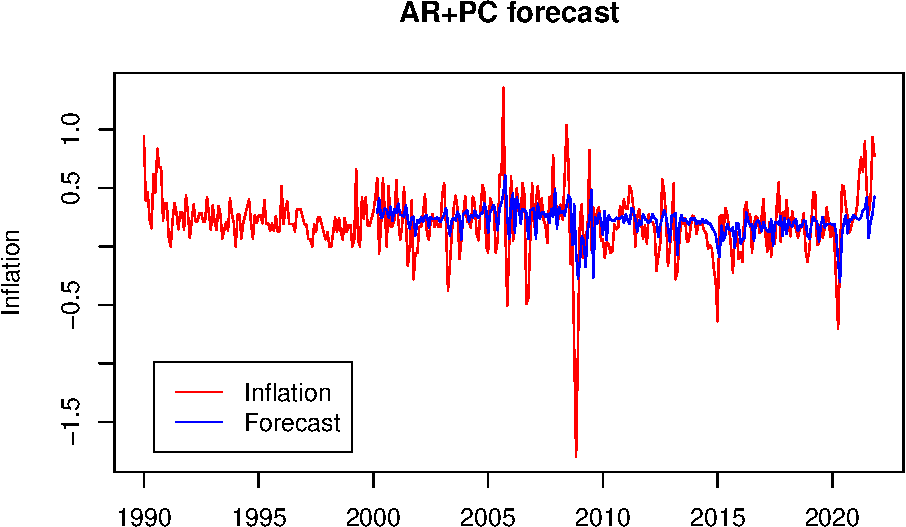
\includegraphics{Trabalho_Econo4_Q3_files/figure-latex/unnamed-chunk-5-1.pdf}

\hypertarget{item-e}{%
\subsection{Item E}\label{item-e}}

\begin{Shaded}
\begin{Highlighting}[]
\CommentTok{\# Forecasting error}
\NormalTok{forecasts }\OtherTok{=} \FunctionTok{cbind}\NormalTok{(forecasts\_Q2, }\AttributeTok{RF =}\NormalTok{ forecast1) }\SpecialCharTok{\%\textgreater{}\%}
    \FunctionTok{as.ts}\NormalTok{()}
\NormalTok{error }\OtherTok{=}\NormalTok{ inflation }\SpecialCharTok{{-}}\NormalTok{ forecasts}
\NormalTok{cum\_error }\OtherTok{=}\NormalTok{ error }\SpecialCharTok{\%\textgreater{}\%}
    \FunctionTok{data.frame}\NormalTok{() }\SpecialCharTok{\%\textgreater{}\%}
    \FunctionTok{mutate\_all}\NormalTok{(}\ControlFlowTok{function}\NormalTok{(x) \{}
\NormalTok{        (x}\SpecialCharTok{\^{}}\DecValTok{2}\NormalTok{) }\SpecialCharTok{\%\textgreater{}\%}
            \FunctionTok{cumsum}\NormalTok{()}
\NormalTok{    \}) }\SpecialCharTok{\%\textgreater{}\%}
    \FunctionTok{bind\_cols}\NormalTok{(}\AttributeTok{date =}\NormalTok{ zoo}\SpecialCharTok{::}\FunctionTok{as.Date.yearmon}\NormalTok{(}\FunctionTok{time}\NormalTok{(error))) }\SpecialCharTok{\%\textgreater{}\%}
    \FunctionTok{setNames}\NormalTok{(}\FunctionTok{c}\NormalTok{(}\StringTok{"AR"}\NormalTok{, }\StringTok{"AR\_PC"}\NormalTok{, }\StringTok{"RF"}\NormalTok{, }\StringTok{"date"}\NormalTok{))}
\end{Highlighting}
\end{Shaded}

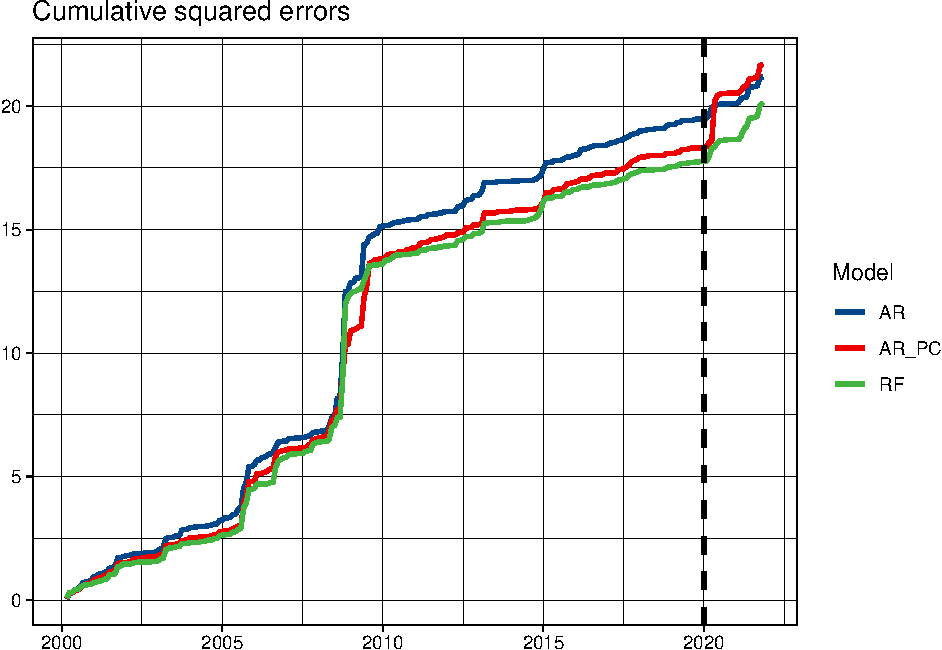
\includegraphics{Trabalho_Econo4_Q3_files/figure-latex/unnamed-chunk-7-1.pdf}

\begin{Shaded}
\begin{Highlighting}[]
\NormalTok{beepr}\SpecialCharTok{::}\FunctionTok{beep}\NormalTok{()}
\end{Highlighting}
\end{Shaded}


\end{document}
